\chapter{Laserová projekce}
Laserová projekce spadá mezi laser scanning technologie. Často je~využívána v~zábavním průmyslu, hlavně k~vytváření laser shows a~vektorových projekcí. U~laser shows diváci sledují vzory, které vytváří samotný paprsek ve~vzduchu. U~projekcí diváci sledují obrazce vykreslené paprskem dopadajícím na~promítací plátno.~\cite{laser-projection}

Tyto efekty nejsou populární pouze v~klubech, nýbrž i~na~koncertech nebo živých představeních. Je-li laser dostatečně silný, je~možné promítat na~obrovské plochy, jako například hráze, vodní plochy, nebo dokonce hory.~\cite{laser-projection} \fxnote{myslim, ze~poměr stupňovací - s~carkou}

\section{Využití laserové projekce v~průhledových displejích~(HUD)}
Laserová projekce se~také využívá v~průhledových displejích. Příklady HUD~jsou vidět na~obrázcích~\ref{fig:hud} a~\ref{fig:hudd}.


\begin{figure}[h]
  \centering
  \begin{minipage}{0.45\textwidth}
    \centering
    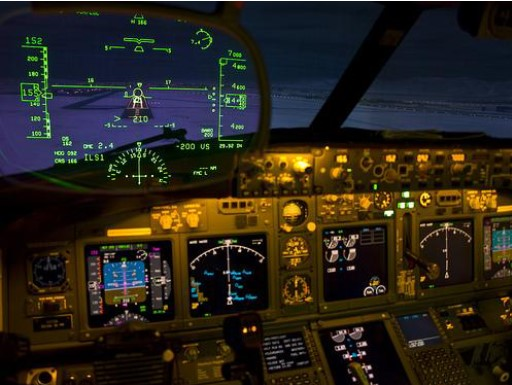
\includegraphics[width=0.9\textwidth]{img/hud.jpg}
    \caption{\label{fig:hud} HUD~v letadle Boeing 737-800~\cite{dev-of-laser-huds-in-driving}}
  \end{minipage}\hfill
  \begin{minipage}{0.45\textwidth}
    \centering
  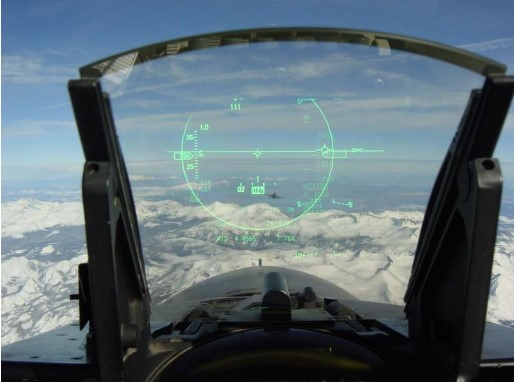
\includegraphics[width=0.9\textwidth]{img/hudd.jpg}
  \caption{\label{fig:hudd} HUD~ve stíhacím letounu F16~\cite{dev-of-laser-huds-in-driving}}
  \end{minipage}
\end{figure}

% \begin{figure}[h]
%   \centering
%   \begin{minipage}{0.45\textwidth}
%     \centering
%   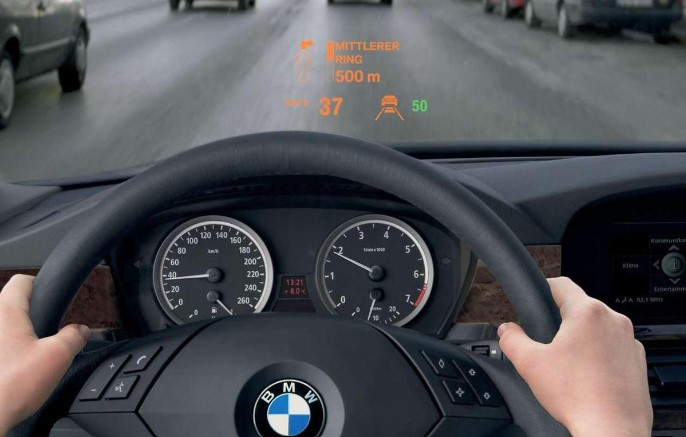
\includegraphics[width=0.9\textwidth]{img/huddd.jpg}
%   \caption{\label{fig:huddd} HUD~v automobilu BMW~5-series~\cite{dev-of-laser-huds-in-driving}}
% \end{minipage}\hfill
% \begin{minipage}{0.45\textwidth}
%   \centering
%   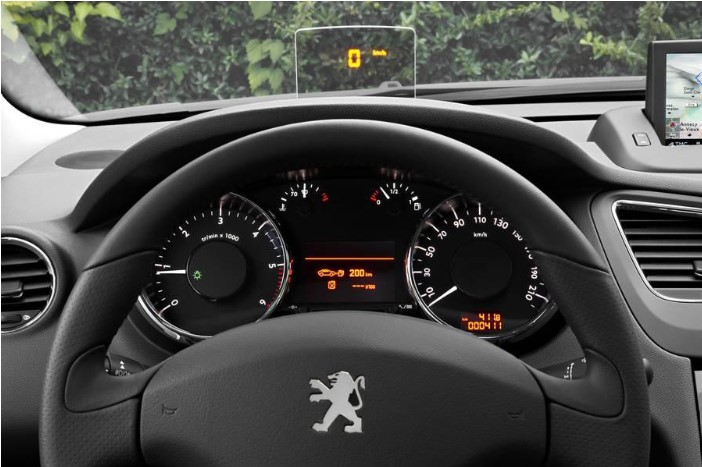
\includegraphics[width=0.9\textwidth]{img/hudddd.jpg}
%   \caption{\label{fig:hudddd} HUD~v automobilu Peugeot 5008~\cite{dev-of-laser-huds-in-driving}}
% \end{minipage}
% \end{figure}

V~tomto odvětví zatím převládají jiné technologie. Technologie průhledových displejů se~dají rozdělit následovně:
\begin{itemize}
  \item Technologie vyzařujících displejů,~např. cathode ray~tube~(CRT), organic light-emitting diode~(OLED) nebo vacuum fluorescent display (VFD).
  \item Technologie podsvícených displejů,~např. liquid crystal display (LCD).
  \item Technologie laserových displejů,~např. liquid crystal on~silicon (LCoS) nebo laser scanning displeje založené na~pohybu mikrozrcadel.~\cite{dev-of-laser-huds-in-driving}
\end{itemize}

V prvních průhledových displejích bylo využito CRT. Ale~kvůli své neskladnosti, vysoké spotřebě elektřiny a~škodlivé radiaci, byla nahrazena technologií LCD. Dnes se~v~průhledových displejích letadel využívají LCD. V~automobilech se~využívají LCD~a~VFD.
Bohužel VFD~jsou limitovány množstvím informací, které mohou zobrazit. LCD~průhledové displeje jsou limitovány svým maximálním jasem.
S novou technologií OLED sice je~možné vytvořit tenký a~průhledný displej dosahující vyšího jasu než LCD~HUD.
I tento displej bohužel oproti vnějšímu světu má stále relativně nízký jas, také má vysokou cenu a~krátkou životnost.
Oproti vyzařujícím a~podsvíceným displejům jsou laserové displeje nadřazené.~\cite{dev-of-laser-huds-in-driving}

\section{Princip laserové projekce}\label{sec:projection-princip}
Když se~laserový paprsek pohybuje dostatečně rychle, lidské oko~ho~vnímá jako spojitou linku světla -- tomuto jevu se~říká \It{persistance of~vision} nebo \It{persistance of~impression}~\cite{persistance-of-vision}.
Čím rychleji se~paprsek pohybuje, tím méně intenzivní připadá oku~zmíněná linka. Bod~je~možné vykreslit, jestliže paprsek zůstane na~jednom místě bez~pohybu po~úrčitou dobu.~\cite{laser-projection}

Vykreslení čáry je~základní a~nejjednoduší operací, jakou laserový projektor může vykonat. Například k~vykreslení úsečky z~bodu A~do~bodu B~projektor nasměřuje laserový paprsek na~bod~A, zapne laser a~pohybuje paprskem k~bodu B.~\cite{laser-projection}

K vykreslení složitějších obrázků jsou potřeba tzv. blank\ lines, kdy~projektor otáčí zrcátky stejně, jako kdyby vykresloval přímku, ale~laser nesvítí. Blank lines spojují každé dvě vykreslené linky, které na~sebe přímo nenavazují.~\cite{laser-projection}

Nestihne-li projektor vykreslovat obraz dostatečně rychle, výsledná projekce nebude stabilní. Lidské oko~vždy uvidí pouze části obrazu v~časové návaznosti. Tomuto jevu se~říká \uv{flickering}.~\cite{laser-projection}

Příklad obrazu vykresleného laserovým projektorem je vidět na obrázku~\ref{fig:gyrec}. Na tomto obrázku foto aparát zachytil i částečný \uv{flickering}, pro lidské oko ovšem nebyl viditelný.

\begin{figure}[htb]
  \centering
  \includegraphics[width=1\textwidth]{img/gyrec.JPG}
  \caption{\label{fig:gyrec} Ukázka projekce; doba závěrky fotoaparátu 1/30~s}
\end{figure}